\documentclass[Afour,sageh,times]{sagej}
\usepackage[utf8]{inputenc}
\usepackage[USenglish]{babel}
\usepackage{booktabs}
\usepackage{setspace}
\usepackage{csquotes}
\usepackage{url}
\usepackage{moreverb}
\usepackage[colorlinks,bookmarksopen,bookmarksnumbered,citecolor=red,urlcolor=red]{hyperref}
\newcommand\BibTeX{{\rmfamily B\kern-.05em \textsc{i\kern-.025em b}\kern-.08em T\kern-.1667em\lower.7ex\hbox{E}\kern-.125emX}}


\def\volumeyear{\the\year}




\begin{document}

\runninghead{Author Redacted}
\title{The Importance of Being Nonplanar: Street Network Representation in Urban Form Studies}
\author{Author Redacted \affilnum{1}}
\affiliation{\affilnum{1}Affiliation redacted}
\corrauth{Author Redacted, Address Redacted}
\email{Email Redacted}


\begin{abstract}

\end{abstract}

\keywords{street network, GIS, urban form, transportation, urban design}

\maketitle

\section{Introduction}

In urban planning and design research, street networks are routinely used to calculate accessibility between origins and destinations or to compute indicators of the urban form, such as block sizes or intersection density and connectivity. Mathematical models of street networks, called graphs, have grown ubiquitous in the urban studies literature in recent years as they have been used to model household travel patterns, access and equity, pedestrian volume, urban design patterns and spatial morphology, and location centrality and polycentricity \citep{marshall_street_2010,porta_alterations_2014,marshall_community_2014,hajrasouliha_impact_2015,parthasarathi_street_2015,knight_metrics_2015,gil_street_2016,zhong_revealing_2017}.

In the urban studies literature, street networks are typically referred to as \enquote{planar} or \enquote{approximately planar} (see Table \ref{tab:planar_quotes}), meaning that they can be well-modeled by a flat two-dimensional model that inherently forbids overpasses or underpasses. Of course in the real world, urban street networks are embedded in three-dimensional space and often feature grade separation, bridges, and tunnels. This leads to two intertwined questions. First, how well do these planar graphs model urban street networks? Second, what does the extent to which a network is nonplanar tell us about a city's infrastructure and development?

This study tests the planarity of street networks around the world. It also presents two new measures of the degree of nonplanarity that can be generalized to other types of spatial networks. These indicators help describe the nature of the urban form and transportation infrastructure. Despite common claims in the literature that street networks are planar graphs, this study finds that they generally are nonplanar and that planar graphs poorly model the street networks of many cities. Further, the magnitude of this bias varies substantially across cities and urbanization types.

This article is organized as follows. The following section introduces the relevant basics of graph theory in urban studies, focusing on discussions in the research literature about street network planarity. The next section discusses the methods used to acquire and analyze the street networks in this study. Then we present the results of this analysis before concluding with a discussion of their ramifications for street network research and urban form studies.


\section{Background and Motivation}

Graph theory is the mathematical study of networks \citep{newman_networks:_2010}. Graphs can mathematically model real-world networks such as friendships or the Internet as well as spatial networks, such urban street networks \citep{barthelemy_spatial_2011}. A graph $G$ consists of a set of nodes $N$ connected to one another by a set of edges $E$. An edge $uv$ in a directed graph points in one direction from some node $u$ to some node $v$, but an undirected graph's edges all mutually point in both directions. In a street network, the nodes represent intersections and dead-ends, and the (directed) edges represent the street segments that connect them. How a graph's nodes and edges connect to one another defines its \emph{topology}. For example, a node's \emph{degree} is a topological trait that represents how many edges connect to that node. A \emph{planar} graph can be drawn on a two-dimensional plane without any of its edges crossing each other, except where they intersect at nodes. If the graph \emph{cannot} be drawn --- or redrawn --- to meet this criterion, then the graph is nonplanar \citep{trudeau_introduction_1994}. Street networks are embedded in space, which provides them with geometry --- such as geographical coordinates, lengths, and areas --- along with their topology.

\begin{table*}[htbp]
\centering
\caption{Recent statements in the urban studies and urban physics literatures regarding the representation of street networks as planar graphs.}
\label{tab:planar_quotes}
\begin{tabular}{ | p{\textwidth} | }

\hline

\enquote{In a planar graph, no links intersect, except by nodes. This feature represents a transportation network well.} \citep[p.~6]{dill_measuring_2004} \\ \hline

\enquote{Street networks are planar graphs composed of junctions and street segments...} \citep[p.~18]{batty_network_2005} \\ \hline

\enquote{The number of long-range connections and the number of edges that can be connected to a single node are limited by the spatial embedding. This is particularly evident in planar networks e.g., those networks forming vertices whenever two edges cross, as urban streets or ant networks of galleries...} \citep[p.~1]{crucitti_centrality_2006} \\ \hline

\enquote{Any of these street networks (SNS) can be described by an embedded planar graph... Street networks are planar graphs and such planarity strongly constrains their heterogeneity...} \citep[pp.~514~\&~521]{buhl_topological_2006} \\ \hline

\enquote{Planar graphs are those graphs forming vertices whenever two edges cross, whereas nonplanar graphs can have edge crossings that do not form vertices. The graphs representing urban street patterns are, by construction, planar...} \citep[p.~3]{cardillo_structural_2006} \\ \hline

\enquote{The connection and arrangement of a road network is usually abstracted in network analysis as a directed planar graph...} \citep[p.~340]{xie_measuring_2007} \\ \hline

\enquote{Urban street patterns form planar networks... The simplest description of the street network consists of a graph whose links represent roads and whose vertices represent road intersections and end points. For these graphs, links intersect essentially only at vertices and are thus planar.} \citep[p.~1]{barthelemy_modeling_2008} \\ \hline

\enquote{Urban street networks as spatial networks are embedded in planar space, which give many constraints.} \citep[p.~1]{hu_topological_2008} \\ \hline

\enquote{...a street network is a strange network when compared to other social or biological networks in the sense that it is embedded in the Euclidian [sic] space and the edges do not cross each other. In graph theory, such a network is called a planar graph.} \citep[p.~259]{masucci_random_2009} \\ \hline

\enquote{...street networks are embedded in space and are planar in nature...} \citep[p.~114]{porta_networks_2010} \\ \hline

\enquote{Roads, rail, and other transportation networks are spatial and to a good accuracy planar networks. For many applications, planar spatial networks are the most important...} \citep[p.~3]{barthelemy_spatial_2011} \\ \hline

\enquote{...urban road systems can be (in good approximation) considered as planar networks, i.e., links cannot \enquote{cross} each other without forming a physical intersection (node) as long as there are no tunnels or bridges... The meaningful definition of link angles requires the presence of a planar network, which is assumed to be the case in urban road systems.} \citep[pp.~563~\&~567]{chan_urban_2011} \\ \hline

\enquote{Road networks are planar graphs consisting of a series of land cells surrounded by street segments.} \citep[p.~3]{strano_elementary_2012} \\ \hline

\enquote{Planar graphs are basic tools for understanding transportation systems embedded in two-dimensional space, in particular urban street networks... As these graphs are embedded in a two-dimensional surface, the
planarity criteria requires that the links do not cross each other.} \citep[p.~1]{masucci_limited_2013} \\ \hline

\enquote{...street networks are essentially planar; in the absence of tunnels and bridges, the streets (the links) cannot cross without generating an intersection or a junction, that is, a node.} \citep[p.~1]{gudmundsson_entropy_2013}. \\ \hline

\enquote{Networks of street patterns belong to a particular class of graphs called planar graphs, that is, graphs whose links cross only at nodes.} \citep[p.~1074]{strano_urban_2013} \\ \hline

\enquote{In city science, planar networks are extensively used to represent, to a good approximation, various infrastructure networks... in particular, transportation networks and more recently streets patterns...} \citep[p.~1]{viana_simplicity_2013} \\ \hline

\enquote{...finding a typology of street patterns essentially amounts to classifying planar graphs...} \citep[p.~2]{louf_typology_2014} \\ \hline

\enquote{...we are dealing with spatial graphs, which tend to be planar...} \citep[p.~2191]{zhong_detecting_2014} \\ \hline

\enquote{Urban transport systems as networks can be represented as planar graphs...} \citep[p.~2]{wang_resilience_2015} \\ \hline

\enquote{Modeling a road network as a planar graph seems very natural.} \citep[p.~42]{aldous_routed_2016} \\ \hline

\enquote{In city science, planar networks are extensively used to represent various infrastructure networks. In particular, transportation networks and street patterns...} \citep[p.~257]{barthelemy_paths_2017} \\ \hline

\enquote{In graph theory, a spatial street network is a type of planar graph embedded in Euclidean space.} \citep[p.~168]{law_defining_2017} \\ \hline

\end{tabular}

\end{table*}

This creates a minor wrinkle when we consider planarity: we must distinguish between a graph's topological planarity, which we refer to as \emph{formal planarity}, and the planarity of its particular spatial embedding, which we refer to as \emph{spatial planarity}. For example, a street network might be spatially nonplanar due to its embedding in space (i.e., it contains overpasses or underpasses in the real world), but it could still be formally planar. If we \enquote{redraw} the graph by moving its nodes and edges around in space without changing how they are connected to one another (i.e., altering its geometry without altering its topology), there may exist some spatial embedding that prevents edges crossing anywhere but at nodes \citep[for a comprehensive discussion see][pp.~6--10]{barthelemy_morphogenesis_2017}. In such a case, the street network is formally planar from a topological perspective, but its real-world embedding is spatially nonplanar.

Consider two theoretical examples: a medieval European city center and a modern American city center. The former's circulation network comprises a set of pedestrian paths and drivable streets without any grade separation, overpasses, or underpasses. In two-dimensions, its edges (i.e., streets and paths) cross each other only at nodes (i.e., intersections), so it is by definition planar. The latter's circulation network comprises pedestrian paths, drivable surface streets, and a grade-separated freeway with overpasses over some of the surface streets. In two-dimensions, its edges occasionally cross each other at non-nodes (i.e., overpasses), so it is by definition nonplanar. However, we might call it \emph{approximately} planar because its nonplanar edge crossings are relatively uncommon. Approximate planarity constrains nonplanar spatial networks such that they do not exhibit certain characteristics found among nonplanar aspatial graphs (e.g., small-world effects or power-law distributed node degrees).

In the urban studies and urban physics literature, street networks are commonly referred to as planar graphs. Table \ref{tab:planar_quotes} presents a survey of statements and reasoning around this claim. Some authors prefer to hedge slightly, arguing that street networks are \emph{approximately} or \emph{essentially} planar graphs that are close enough to be well-modeled as such.

If street networks can be sufficiently well-modeled by planar graphs, there are certain methodological benefits to doing so. Planar graphs offer computational simplicity and tractability. They enable easy polygonal spatial analysis of city blocks and form \citep{fohl_non-planar_1996} as well as the Euler characteristic. In mathematics, there is a bijection between planar graphs and trees, and classifying planar graphs presents a trivial problem \citep{louf_typology_2014}. Planar graphs are easier to visualize and can be faster to run algorithms on \citep{liebers_planarizing_2001}. Accordingly, \citet[p.~3]{barthelemy_spatial_2011} argues that \enquote{planar spatial networks are the most important and most studies have focused on these examples}. But in contrast, \citet{masucci_random_2009} and \citet{masucci_limited_2013} argue that planar graphs remain a compelling research domain for urban scholars because they were understudied until recently for two reasons: they appear topologically trivial and planarity does not lend itself to certain popular graph-theoretic analyses. Discussing the open research area around street networks as planar graphs, \citet[p.~1]{viana_simplicity_2013} state, \enquote{there is still a lack of global, high-level metrics allowing to characterize their structure and geometrical patterns.}

Despite the computational and mathematical advantages of simple planar models, street networks are often nonplanar in reality: many include at least one overpass or underpass that results in the failure of formal proofs of their planarity, such as the \citet{kuratowski_sur_1930} theorem or the \cite{hopcroft_efficient_1974} algorithm \citep[cf.][]{gastner_spatial_2006}. As \citet[p.~7]{levinson_network_2012} points out, \enquote{Real networks are neither perfect, nor planar, nor grids, though they may approximate them.}

Other authors have commented on this characteristic of street networks. \citet[p.~199]{jiang_object-oriented_2010} explain that \enquote{Quite often the transportation network has overpasses and underpasses that require a non-planar network representation.} \citet[p.~1258]{fischer_spatial_2014} explains that \enquote{For many infrastructure networks, {[planarity]} is approximately true, although bridges and tunnels in ground-transport networks are an obvious (but generally minor) exception.} Twenty years ago, \citep[p.~18]{fohl_non-planar_1996} claimed, \enquote{The most commonly used data model for transportation networks is the fully intersected, planar data model} and called for a nonplanar model to better represent truly nonplanar spatial networks. \enquote{The planar network data model has received widespread acceptance and use. Despite its popularity, the model has limitations for some areas of transportation analysis, especially where complex network structures are involved. One major problem is caused by the planar embedding requirement... intersections at grade cannot be distinguished from intersections with an overpass or underpass that do not cross at grade.} \citep[p.~395]{fischer_gis_2004} 

If a planar graph models a street network poorly, it could do so in multiple ways. Forcing planarity on a nonplanar street network creates artificial nodes at bridges and tunnels, which breaks routing. As \citet[p.~6]{kwan_review_1996} put it, \enquote{the difficulty in accurately representing overpasses or underpasses may lead to problems when running various routing algorithms (e.g. recommending that a traveler make a left-turn at an intersection that proves to be an overpass)}. Second, and accordingly, intersection counts and density will be overestimated by the presence of these pseudonodes. Consequently, edge lengths will be underestimated due to these artificial breakpoints in the middle of street segments. Finally, this bias would likely behave inconsistently across different kinds of cities and street network types.

Given these issues, what do \emph{approximately planar} and \emph{well-modeled} mean for street network research? How close is \enquote{close enough} for a planar graph to competently model a formally nonplanar street network? Do the biases of planar models behave consistently across geographies and development eras or do they misrepresent different cities to different degrees? And if street networks are at least generally approximately planar, how can we measure just how planar or nonplanar a given street network is?

The graph theory literature offers some measures of how \enquote{far off} a nonplanar graph $G$ is from being planar, including its \emph{crossing number} --- the minimum number of edge crossings of any drawing of $G$ --- and its \emph{skewness} --- the minimum number of edges that must be removed from $G$ to produce a planar graph \citep{liebers_planarizing_2001,szekely_successful_2004,chimani_non-planar_2009}. However, these measures are imperfect and hard to compute \citep{chimani_vertex_2012,szekely_successful_2004}. They also fail to account for the size or density of a spatial network. In his discussion of road networks and approximate spatial planarity, \citet[p.~133]{newman_networks:_2010} argues that \enquote{no widely accepted metric for degree of planarity has emerged,} and calls for the development of better indicators.

Such metrics would be particularly useful for street networks, as the extent to which a network is (or is not) planar can characterize the nature of its circulation infrastructure and urban form. For instance, late 20th-century freeway-oriented American cities might exhibit lower planarity than older walkable European cities. What about informal settlements in developing countries or rapidly urbanizing Chinese cities? Beyond the question of graph model goodness-of-fit, such indicators could provide useful information about urban development, civil infrastructure, and transportation system character.



\section{Methods}

In this study, we develop two new measures of the extent to which a spatial network is planar. We then analyze various world cities to better understand how well planar graphs model their street networks as well as the extent to which bias (i.e., model misrepresentation) varies across different places and types of urbanization. Finally, we consider what these indicators suggest about the nature of the urban form and transportation infrastructure in different cities.

\subsection{Data}

Following \citet{jacobs_great_1995} and \citet{cardillo_structural_2006}, we analyze a consistently sized, square-mile network at the centers of 50 cities worldwide. This allows us to consistently examine central urban street networks without being swamped by metropolitan-scale variation or the idiosyncrasies of individual municipalities' spatial extents. For cities such as Moscow, with a newer commercial central business district (CBD) that lies apart from an \enquote{old town} center, we use the modern CBD as the city center. We look separately at each city's drivable and walkable street networks.

To acquire these street networks, we use OSMnx to download the data for each city and network type from OpenStreetMap. OpenStreetMap is a collaborative online mapping platform commonly used by researchers because of its good worldwide coverage \citep{haklay_how_2010,jokar_arsanjani_openstreetmap_2015}. OSMnx is a Python-based software tool that allows us to automatically download a street network from OpenStreetMap for any study site in the world, and automatically process it into a length-weighted nonplanar directed graph \citep{boeing_osmnx:_2017}. It differentiates between walkable and drivable routes in the circulation network based on individual elements' metadata that describe how the route may be used. Thus the walkable network may contain surface streets, paths through parks, pedestrian passageways between buildings or under roads, and other walkable paths. The drivable network may contain surface streets, grade-separated freeways, and other drivable paths.

OpenStreetMap's raw data contain many interstitial nodes in the middle of street segments (forming an expansion graph) to allow streets to curve through space via a series of straight-line approximations. OSMnx automatically simplifies each graph's topology to retain nodes only at intersections and dead-ends, while faithfully retaining each edge's true spatial geometry. This provides us with an accurate count of intersections and an accurate measure of edge lengths for comparison between the planar and nonplanar representations of our networks.

\subsection{Analysis}

Once we have acquired and prepared our networks, we calculate three measures of planarity. The first is an aspatial test of formal planarity using the algorithm described by \citet{boyer_subgraph_2012}. That is, is it possible to rearrange the graph's nodes and edges in space --- while preserving its topology --- so that edges cross only at nodes? This binary true/false indicator tells us if the graph is formally planar, ignoring its real-world spatial embedding. However, street networks are spatially embedded, so we develop the following two continuous indicators to assess the \enquote{extent} to which they are planar.

The second measure is the spatial planarity ratio (SPR). It represents the ratio of nonplanar intersections (i.e., non-dead-end nodes in the nonplanar, three-dimensional, spatially-embedded graph) to planar intersections (i.e., line crossings in the planar, two-dimensional, spatially-embedded graph). This indicates the extent to which planarity overstates intersections and connectivity in each street network. A truly planar network with no bridges or tunnels will thus have an SPR score of 1.0, while lower values indicate the extent to which the network is nonplanar.

The third measure is the edge length ratio (ELR). It represents the ratio of the mean edge length in the planar graph to the mean edge length in the nonplanar graph. This indicates the extent to which planarity understates edge lengths in each street network. A truly planar street network with no bridges or tunnels will thus have an ELR score of 1.0, while lower values indicate the extent to which the network is nonplanar.

Finally, we explore how these indicators might vary across a single municipality. To do so we analyze the drivable street network of Oakland, California, a reasonably representative midsized American city with a variety of urban form types from gridded street patterns in its flatlands, to winding culs-de-sac in its hills, to freeways and dense blocks around its downtown. First we analyze the entire city of Oakland. Then we recreate the aforementioned methodology by randomly sampling 100 points within the city limits and analyzing the square-mile street networks centered on each. The resulting statistical dispersion of planarity indicators demonstrates the extent to which agglomerating an entire city's neighborhoods into a single graph may obscure neighborhood-scale effects and characteristics.




\section{Results}

\subsection{Worldwide Cities}

\begin{table*}[htbp]
	\centering
	\caption{Planarity measures for the central street networks of 50 cities worldwide (SPR = spatial planarity ratio; ELR = edge length ratio; Planar = whether street network passed the formal test of planarity).}
	\label{tab:world_cities}
	\begin{tabular}{ l l r r r r r r  }
\toprule
             &               & \multicolumn{3}{|c|}{Drive}         & \multicolumn{3}{c}{Walk}            \\
\midrule
Country      & City          &  Planar  &  $\phi$   &  $\lambda$   &  Planar  &  $\phi$   &  $\lambda$   \\
\midrule
Argentina & Buenos Aires &      Yes &  1.000 &  1.000 &       No &  0.946 &  0.947 \\
Australia & Sydney &       No &  0.741 &  0.749 &       No &  0.909 &  0.901 \\
Brazil & Sao Paulo &       No &  0.791 &  0.790 &       No &  0.852 &  0.831 \\
Canada & Toronto &      Yes &  0.930 &  0.958 &       No &  0.858 &  0.848 \\
          & Vancouver &       No &  0.929 &  0.948 &       No &  0.929 &  0.926 \\
Chile & Santiago &       No &  0.875 &  0.887 &       No &  0.972 &  0.971 \\
China & Beijing &       No &  0.818 &  0.872 &       No &  0.842 &  0.848 \\
          & Hong Kong &       No &  0.846 &  0.835 &       No &  0.840 &  0.818 \\
          & Shanghai &       No &  0.682 &  0.717 &       No &  0.670 &  0.659 \\
Denmark & Copenhagen &      Yes &  0.992 &  0.988 &       No &  0.991 &  0.987 \\
Egypt & Cairo &       No &  0.900 &  0.916 &       No &  0.918 &  0.906 \\
France & Lyon &       No &  0.991 &  0.989 &       No &  0.960 &  0.957 \\
          & Paris &       No &  0.988 &  0.993 &       No &  0.920 &  0.917 \\
Germany & Berlin &       No &  0.939 &  0.950 &       No &  0.943 &  0.936 \\
India & Delhi &      Yes &  1.000 &  1.000 &      Yes &  0.993 &  0.992 \\
Indonesia & Jakarta &      Yes &  0.983 &  0.986 &       No &  0.962 &  0.960 \\
Iran & Tehran &       No &  0.962 &  0.973 &       No &  0.957 &  0.956 \\
Italy & Bologna &      Yes &  1.000 &  1.000 &      Yes &  0.996 &  0.996 \\
          & Florence &      Yes &  1.000 &  1.000 &       No &  0.980 &  0.978 \\
          & Milan &      Yes &  1.000 &  1.000 &       No &  0.875 &  0.860 \\
Japan & Osaka &       No &  0.868 &  0.871 &       No &  0.951 &  0.949 \\
          & Tokyo &       No &  0.927 &  0.923 &       No &  0.922 &  0.912 \\
Kenya & Nairobi &       No &  0.974 &  0.974 &       No &  0.949 &  0.943 \\
Mexico & Mexico City &       No &  0.940 &  0.952 &       No &  0.913 &  0.917 \\
Nigeria & Lagos &       No &  0.952 &  0.967 &       No &  0.988 &  0.987 \\
Peru & Lima &       No &  0.939 &  0.941 &       No &  0.932 &  0.931 \\
Philippines & Manila &       No &  0.946 &  0.953 &       No &  0.906 &  0.895 \\
Russia & Moscow &       No &  0.574 &  0.680 &       No &  0.856 &  0.858 \\
Singapore & Singapore &       No &  0.868 &  0.874 &       No &  0.899 &  0.890 \\
Somalia & Mogadishu &      Yes &  1.000 &  1.000 &      Yes &  1.000 &  1.000 \\
South Africa & Johannesburg &       No &  0.851 &  0.883 &       No &  0.997 &  0.997 \\
Spain & Barcelona &      Yes &  1.000 &  1.000 &       No &  0.904 &  0.900 \\
Switzerland & Geneva &       No &  0.985 &  0.982 &       No &  0.828 &  0.813 \\
Thailand & Bangkok &       No &  0.988 &  0.988 &       No &  0.993 &  0.989 \\
Turkey & Istanbul &       No &  0.975 &  0.982 &       No &  0.980 &  0.978 \\
UAE & Dubai &       No &  0.685 &  0.722 &       No &  0.860 &  0.850 \\
UK & Edinburgh &       No &  0.973 &  0.968 &       No &  0.988 &  0.988 \\
          & London &       No &  0.979 &  0.981 &       No &  0.865 &  0.847 \\
USA & Atlanta &       No &  0.736 &  0.777 &       No &  0.738 &  0.724 \\
          & Chicago &       No &  0.776 &  0.814 &       No &  0.807 &  0.804 \\
          & Cincinnati &       No &  0.730 &  0.757 &       No &  0.931 &  0.927 \\
          & Dallas &       No &  0.598 &  0.650 &      Yes &  0.963 &  0.959 \\
          & Los Angeles &       No &  0.583 &  0.635 &       No &  0.793 &  0.799 \\
          & Miami &       No &  0.647 &  0.662 &       No &  0.964 &  0.961 \\
          & New York &       No &  0.881 &  0.901 &       No &  0.942 &  0.941 \\
          & Phoenix &       No &  0.955 &  0.962 &       No &  0.979 &  0.977 \\
          & San Francisco &       No &  0.935 &  0.941 &       No &  0.948 &  0.944 \\
          & Seattle &       No &  0.732 &  0.779 &       No &  0.933 &  0.926 \\
          & Washington DC &       No &  0.948 &  0.956 &       No &  0.967 &  0.967 \\
Venezuela & Caracas &       No &  0.953 &  0.957 &      Yes &  1.000 &  1.000 \\
\bottomrule
\end{tabular}
\end{table*}

Table \ref{tab:world_cities} presents the results of the analysis of the 50 cities worldwide.

Among drivable street networks, only x\% pass the formal test of planarity. On average, they are only x\% planar by the SPR measure and x\% planar by the ELR measure. SPR values range from a high of 1.0 in x cities to a low of 57\% in Moscow. ELR values range from a high of 1.0 in x cities to a low of 64\% in Los Angeles.

Among walkable street networks, only x\% pass the formal test of planarity. On average, they are only x\% planar by the SPR measure and x\% planar by the ELR measure. SPR values range from a high of 1.0 in x cities to a low of 74\% in Atlanta. ELR values range from a high of 1.0 in x cities to a low of 72\% in Atlanta.

\begin{figure*}[htbp]
	\center
	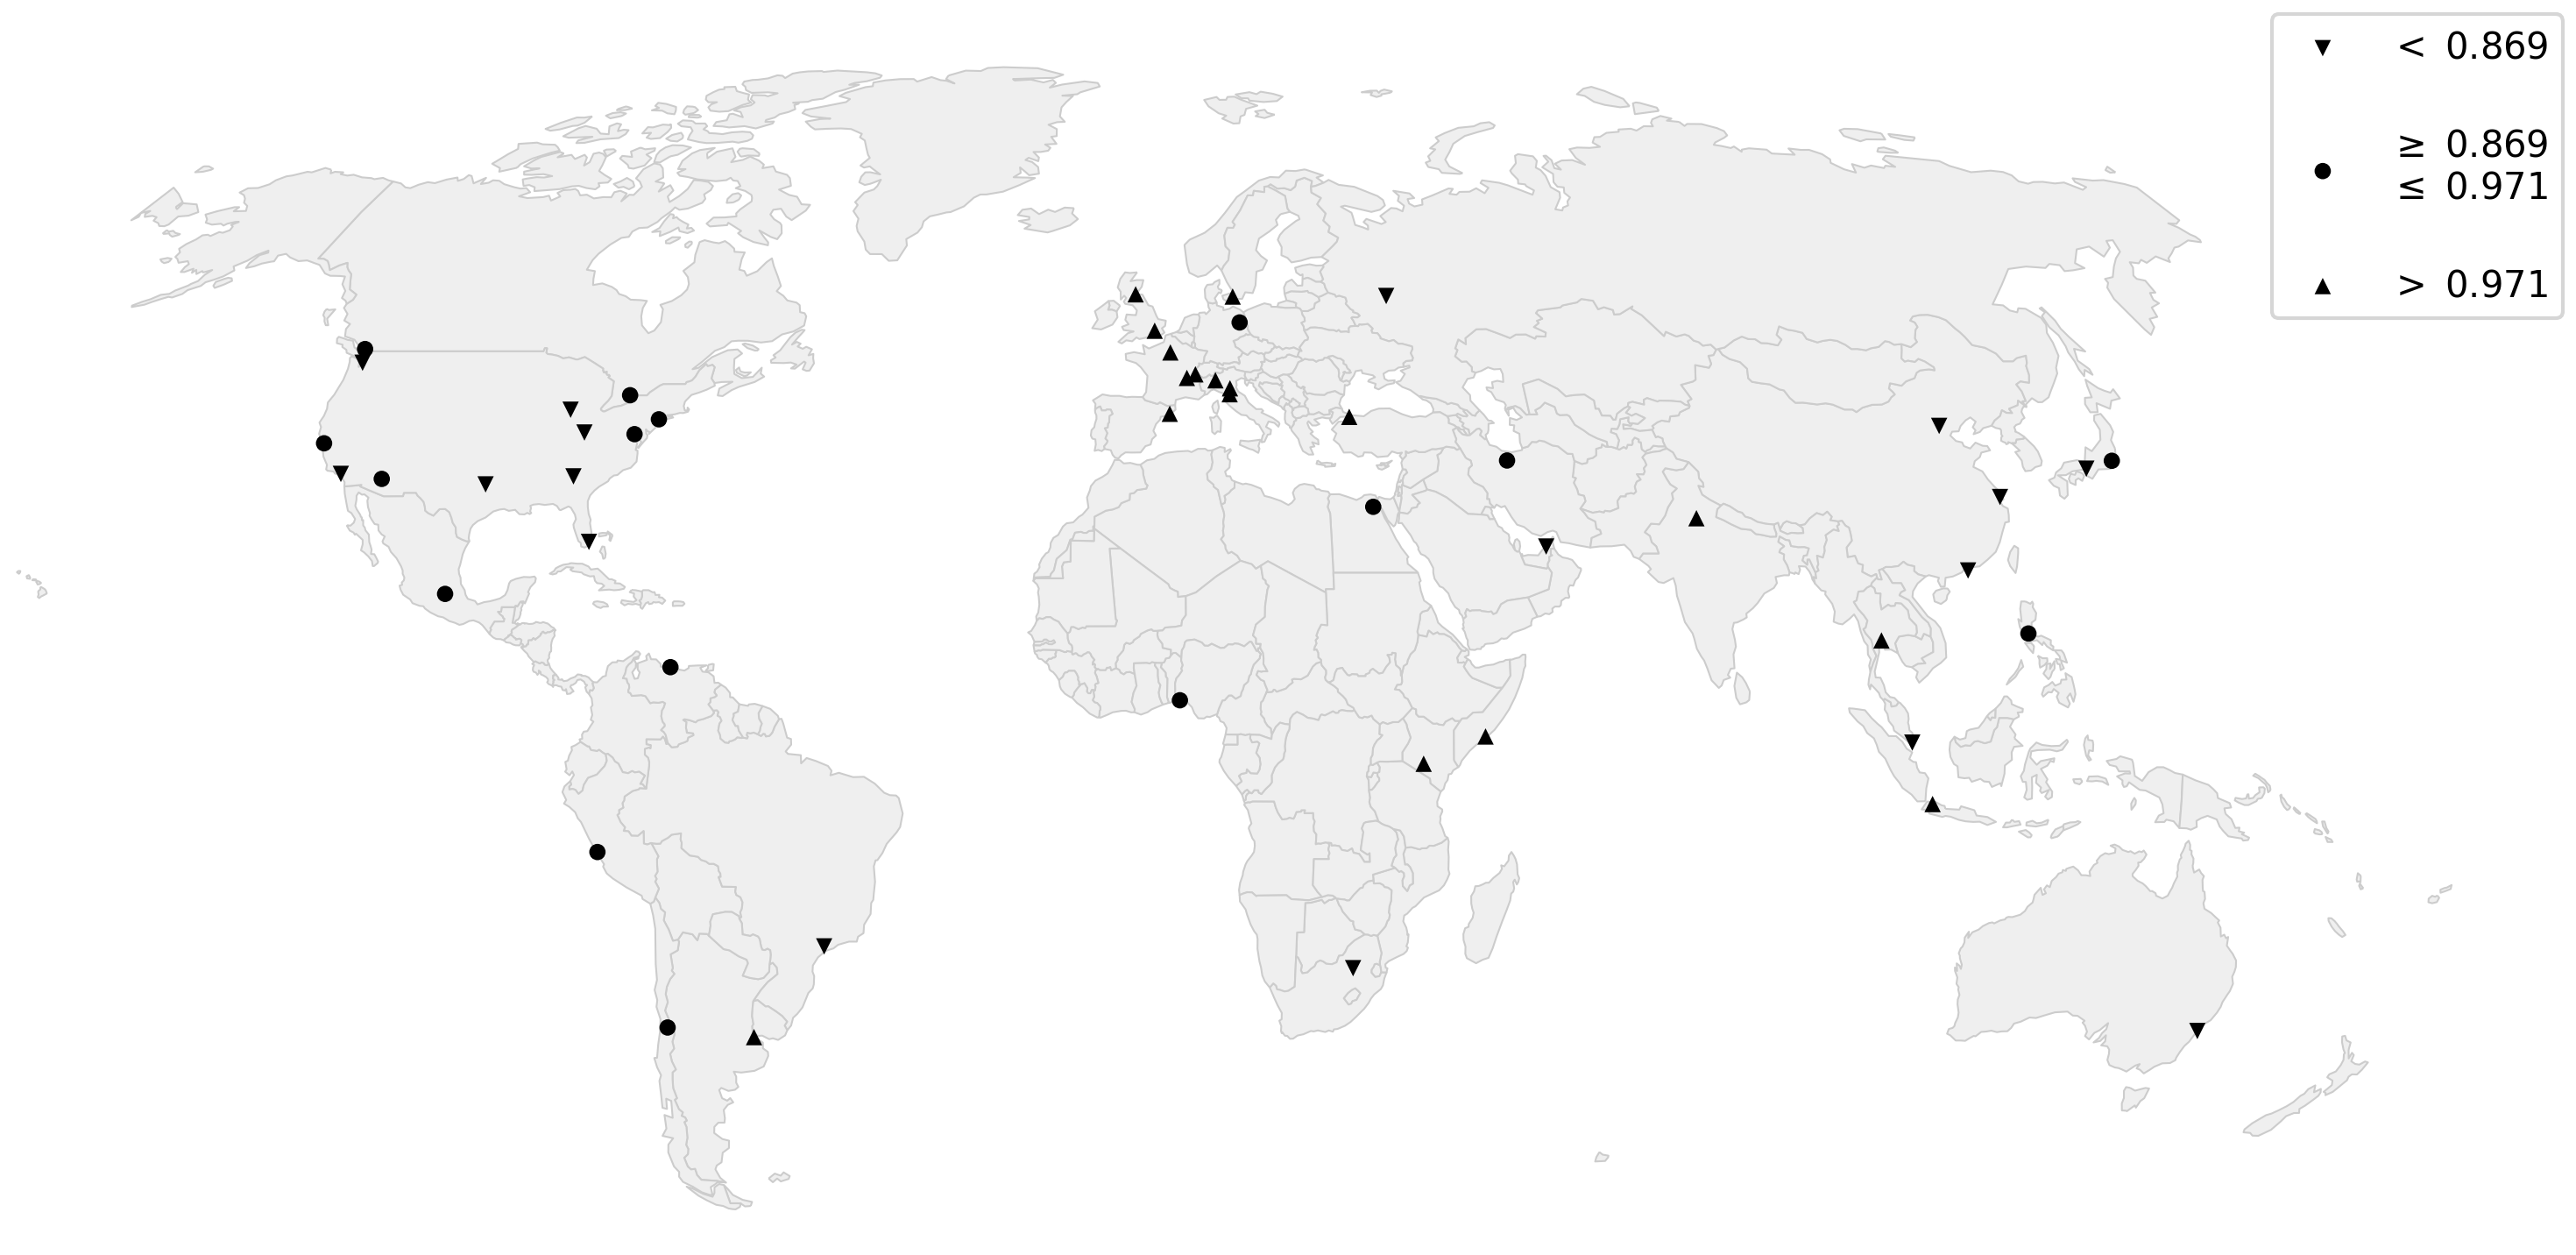
\includegraphics[width=\textwidth]{world_map_phi_bw.png}
	\caption{Map of world cities in Table \ref{tab:world_cities} grouped by SPR score tertiles (lower scores mean less planar).}
	\label{fig:world_map_bw}
\end{figure*}

Figure \ref{fig:world_map_bw} shows the distribution of SPR values around the world. While nearly every European city is in the highest subset, indicating their networks are more planar, most American cities are in the lowest subset, indicating their networks are less planar.

Mogadishu is the only city studied that shows perfect planarity across all three indicators and both network types. All three Italian cities show perfect planarity in their drivable networks, but not in their walkable networks.

\begin{figure}[htbp]
	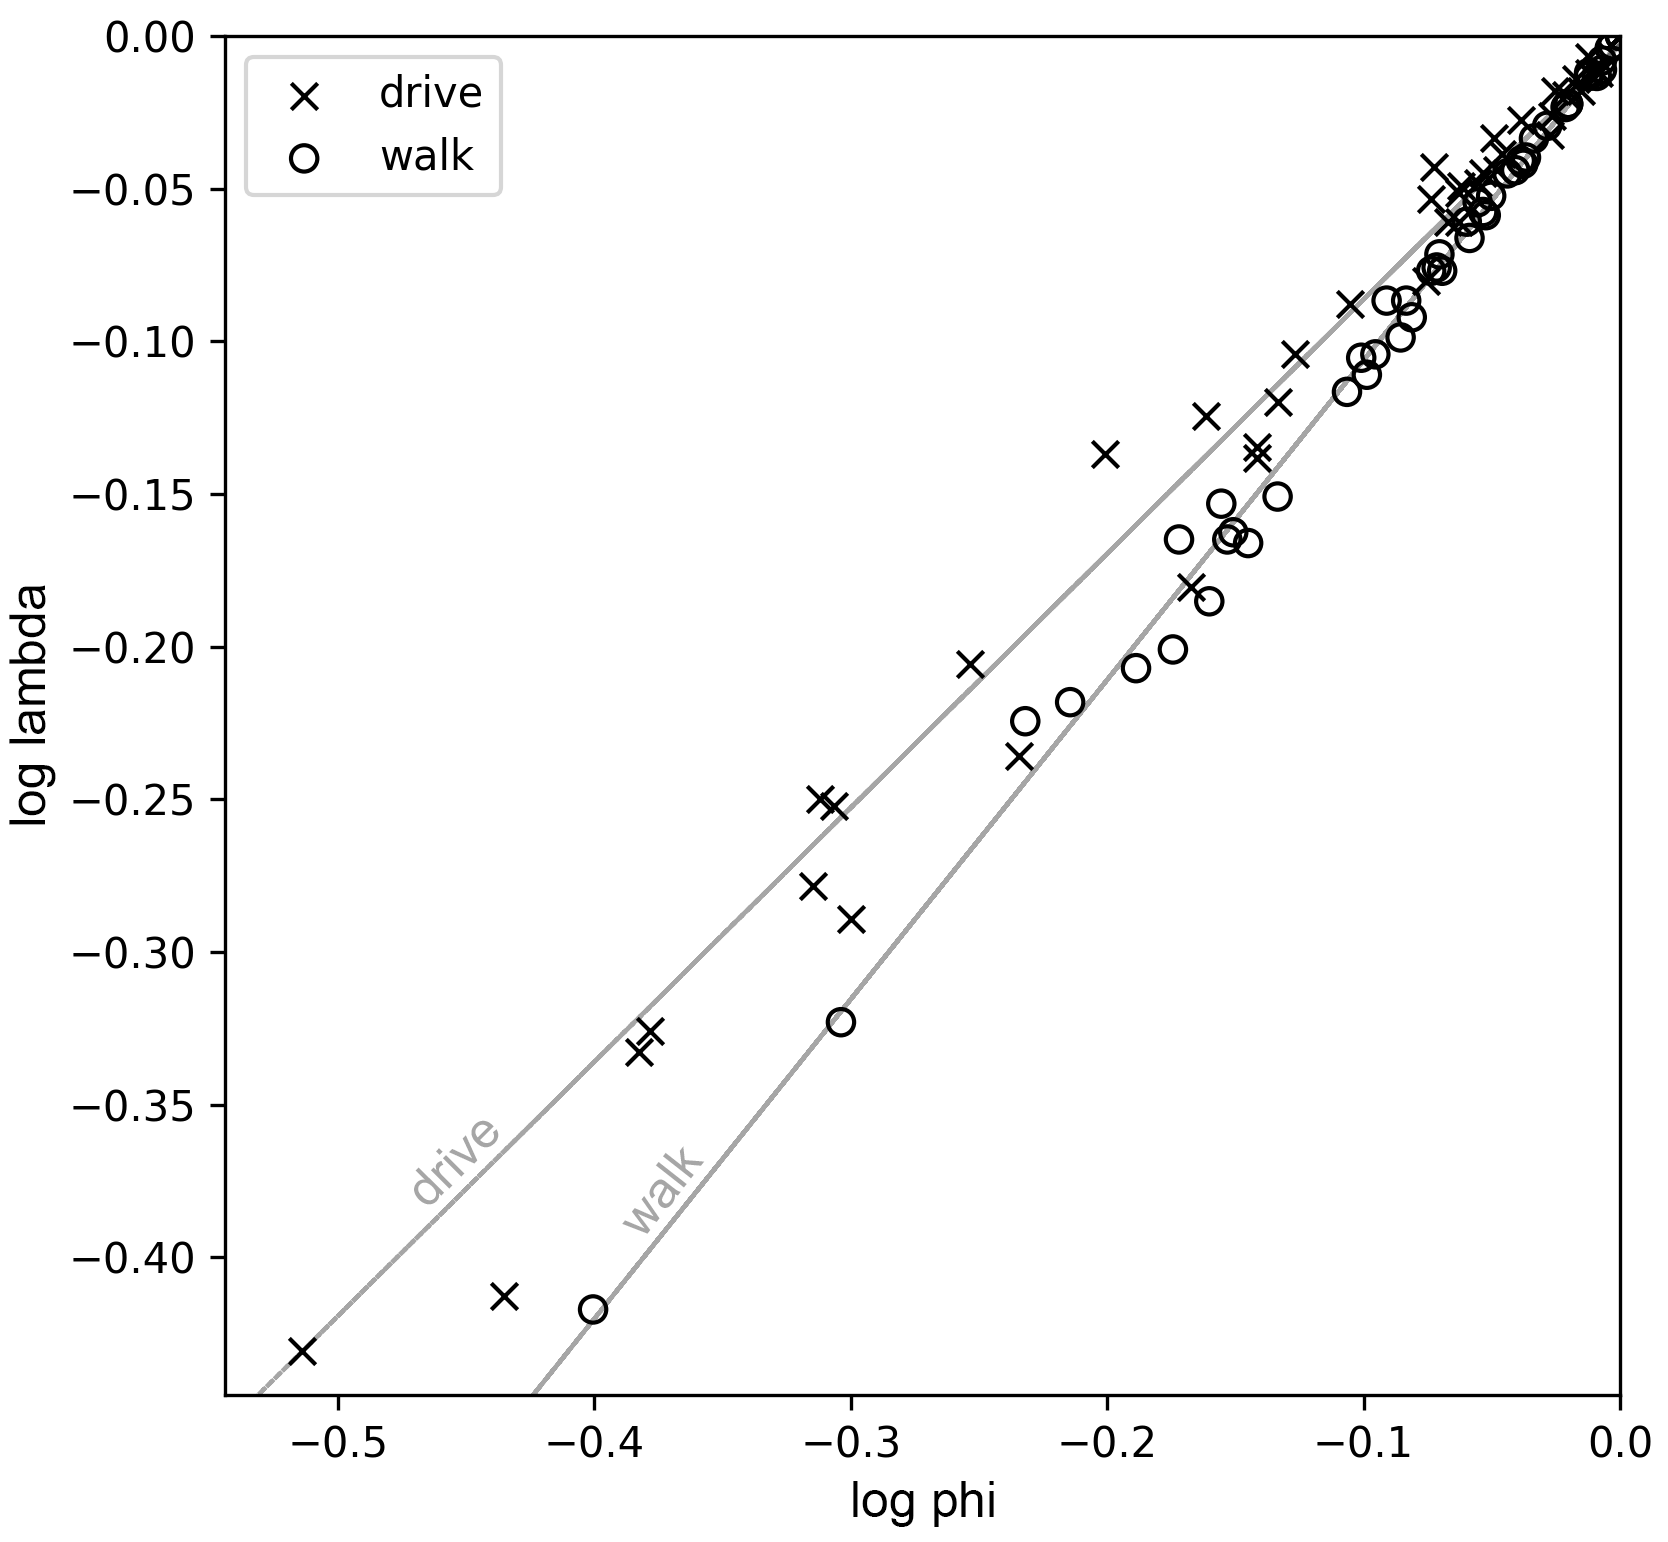
\includegraphics[width=0.48\textwidth]{regression_phi_split.png}
	\caption{Log-log plot of ELR vs SPR with simple regression lines.}
	\label{fig:regression_split}
\end{figure}

Figure \ref{fig:regression_split} shows the relationship between the SPR and ELR indicators across all 50 cities for both network types, as a log-log plot. The indicators' log-log relationship is linear, positive, and very strong (drivable $r^2=0.98$ and walkable $r^2=0.99$).


\subsection{A Closer Look: Oakland, California}

We find that the street network of the entire city of Oakland is formally nonplanar when subjected to a formal mathematical test. In terms of the nonplanarity indicators, the city as a whole has an SPR score of 0.918, indicating that it is 91.8\% planar, and an ELR score of 0.936. This suggests that the planar representation of Oakland's drivable street network overstates the number of intersections (and thus, the network's connectivity) by 8.9\% city-wide (i.e., $1 - 1 / 0.918$ and understates the average edge length by 6.4\% city-wide (i.e., $1 - 0.936$). However, these indicators' values vary across the city.

To explore this statistical variation, we examined 100 square-mile samples of Oakland's drivable street network. Table \ref{tab:samples_city} presents descriptive statistics of these planarity indicators. 



\begin{table}[htbp]
\centering
\caption{Descriptive statistics of planarity indicators across 100 random samples in Oakland, California's drivable network.}
\label{tab:samples_city}
\begin{tabular}{ l r r r r }
\toprule
         &  SPR   &  ELR   \\
\midrule
count	 &    100 &   100  \\
mean     &  0.930 & 0.947  \\
$\sigma$ &  0.101 &  0.082 \\
min      &  0.569 & 0.637  \\
max      &  1.000 & 1.000  \\
\bottomrule
\end{tabular}

\end{table}






\section{Discussion}

Our findings suggest that the street networks in the centers of most major cities are formally and spatially nonplanar. However, this depends on the scale of measurement: across an entire city there is likely to be some underpass or overpass somewhere, while individual neighborhoods or small suburbs might be formally planar. The type and era of urbanization is another factor. Old medieval European towns or informal settlements in the global south contain fewer grade-separated roads (and thus greater planarity) than 20th-century American or 21st-century Chinese metropolises do. This is a result of prevailing transportation technologies when the urban form was built up, as well as terrain, costs, wealth, culture, and politics.

Street networks are frequently nonplanar in the formal sense because they are spatially embedded in three dimensions --- not two --- and have a z-coordinate along with their x and y. Because they are mostly planar, typically with only a few overpasses or underpasses, they could often be described accurately as \emph{approximately planar}. However, claiming that urban street networks broadly are planar misrepresents them in several ways:

\begin{enumerate}
	\item{Forces false nodes where grade-separated edges cross.}
	\item{Accordingly, underestimates average edge length (a proxy for street segment lengths and block sizes).}
	\item{Misrepresents connectivity for routing, accessibility analysis, and other topological studies.}
\end{enumerate}

This is a bigger problem in Los Angeles than in Florence, but even in Florence, planar overcounts intersections around the \textit{sottopassaggio}, or pedestrian subway, near its central train station, Stazione di Santa Maria Novella. This is a pedestrian walkway, not a drivable road, but in a walkable town like Florence, we would surely want to model pedestrian access as part the street network, not drivable roads only. In this case, the nonplanar public pedestrian network must be considered.

The problem is consistently and particularly pronounced around the downtowns of North American cities, due to the prevalence of freeways, bridges, and underpasses there. Driving networks are affected by these in particular. Walking networks are more affected by pedestrian flyovers and subways, as in Florence. Even networks of non-freeway, non-pedestrian-only surface streets will often be nonplanar due to bridges or tunnels in hilly neighborhoods or over rivers.

The effect is inconsistent across cities, and across different neighborhoods within individual cities.

Why are they approximately planar? Cost and politics. Expensive to build truly 3-D networks (with z-coordinates as extensive as their x- and y-coordinates) and politically infeasible.

\subsection{Are street networks planar graphs?}

Contrary to some of the statements in the urban studies and urban physics literature, our results suggest that this cannot be universally claimed. But perhaps some of it comes down to vocabulary. If road is not synonymous with street, then a road network and a street network may not be synonymous. A road network, including freeways and boulevards, may frequently be nonplanar, but a street network, focusing on municipal streets lined by land parcels, may be at-grade and planar. But this ignores the fact that even residential streets sometimes include bridges and tunnels in hilly neighborhoods, and the fact that our analysis earlier showed that walkable circulation networks in city centers often include pedestrian tunnels and footbridges. A graph is not planar because its edges \emph{usually} or \emph{approximately} intersect only at nodes: it is planar because its edges \emph{exclusively} intersect at nodes. Thus, street networks are not universally planar graphs. 

\subsection{Are street networks well-modeled by planar graphs?}

As George Box famously stated, \enquote{All models are wrong but some are useful.} Can street networks be simplified to planar graphs and still be usefully well-modeled? The answer depends on the study site and on the type of analysis. In limited circumstances, where the circulation network and built form exhibit few underpasses, overpasses, or grade-separation, then perhaps yes. But universally, we cannot answer yes.

Most egregiously, imposing planarity on a nonplanar street network forces pseudonodes at underpasses and overpasses, breaking routing and network-based accessibility modeling. For this reason, nonplanar graphs have been the standard for decades in transportation engineering, real-world traffic assignment models, and routing engines.

But planar graphs are often used in the literature to study urban form and morphology. So, aside from routing, do planar graphs offer \emph{useful} models for this type of research? Again, only in limited circumstances, including examples such as the drivable networks in the three Italian cities we analyzed, which are both formally and spatially planar. The results in Table \ref{tab:world_cities} show how common urban form measures such as intersection counts are overstated by planar models, while average edge lengths (a linear proxy for block size) is consequently understated. Moreover, this misrepresentation behaves inconsistently from place to place. Figure \ref{fig:world_map_bw} demonstrates how the magnitude of bias varies across cities and eras of urbanization.

So then why use planar graphs? Tractable. In some cities it doesn't matter (Italy). Polygonal analysis of urban blocks. Otherwise use nonplanar, new tools make it easy.


\section{Conclusion}

Urban researchers frequently use planar graphs to model street networks. This study demonstrated that, although in limited circumstances these models may be accurate, they behave inconsistently across different kinds of cities by misrepresenting connectivity, accessibility, routing, intersection counts and densities, and street segment lengths. It found x, y, and z. It also demonstrated how these indicators can be used to characterize the type of urbanization, in particular transportation infrastructure's three-dimensionality, in different cities. Future research can explore this latter finding, as it likely correlates with other measures of urbanization, development, and era. Finally, future research might examine how nonplanar intersection counts represent true intersections if multiple adjacent edges form multiple graph intersections at a point where only one true intersection exists from an urban design perspective.


%\clearpage
\bibliographystyle{apa}
\bibliography{references}

\end{document}
